
\section{Context}
Here we will be training three different models on the training dataset and testing the performance of the trained model on a test dataset. The feature selection for the dataset is varied from 3 features to 12 features out of maximum 15 features and their results are shown as below.

\subsection{Best 3 features}
Best 3 features as per our model are standard deviation, skewness and RMS value as per our anova test.

\subsubsection{ANN}

\begin{figure}[H]
  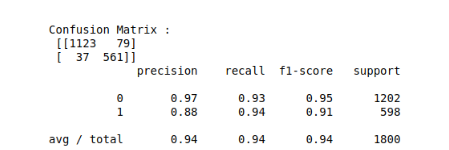
\includegraphics[height = 4cm,width= 9cm]{images/3_feat_ANN}
   \caption{Confusion Matrix for ANN}
\end{figure}

\subsubsection{SVM}

\begin{figure}[H]
  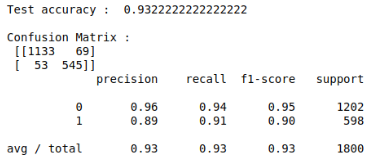
\includegraphics[height = 4cm,width= 9cm]{images/3_feat_SWM}
  \caption{Confusion Matrix for SVM}  
  \end{figure}

\subsubsection{Random Forest}

\begin{figure}[H]
  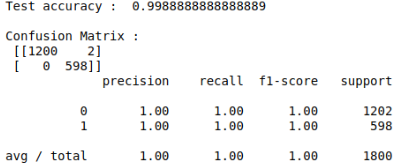
\includegraphics[height = 4cm,width= 9cm]{images/3_feat_rand}
  \caption{Confusion Matrix for Random Forest}
\end{figure}

\subsubsection{Pair Plots}

\begin{figure}[H]
  \noindent\makebox[\textwidth]{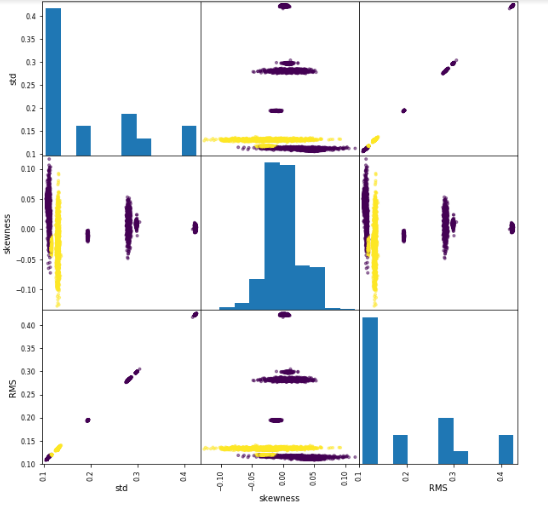
\includegraphics[width=\paperwidth]{images/pairplots_3}}
\caption{Pair plots for 6 features}
\end{figure}


\subsection{Best 6 features}
Best 6 features as per our model are standard deviation, skewness, RMS value, max, pk-pk, and Margin factor as per our anova test.

\subsubsection{ANN}

\begin{figure}[H]
  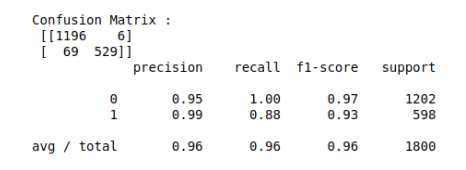
\includegraphics[height = 4cm,width= 9cm]{images/6_ANN}
\caption{Confusion Matrix for ANN}
\end{figure}

\subsubsection{SVM}

\begin{figure}[H]
  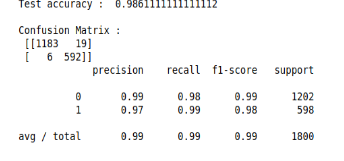
\includegraphics[height = 4cm,width= 9cm]{images/6_SWM}
\caption{Confusion Matrix for SVM}  
  \end{figure}

\subsubsection{Random Forest}

\begin{figure}[H]
  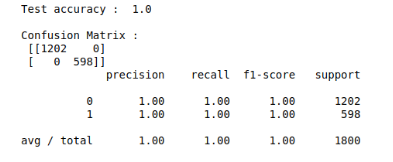
\includegraphics[height = 4cm,width= 9cm]{images/6_rand}
\caption{Confusion Matrix for Random Forest}
\end{figure}

\subsubsection{Pair Plots}

\begin{figure}[H]
  \noindent\makebox[\textwidth]{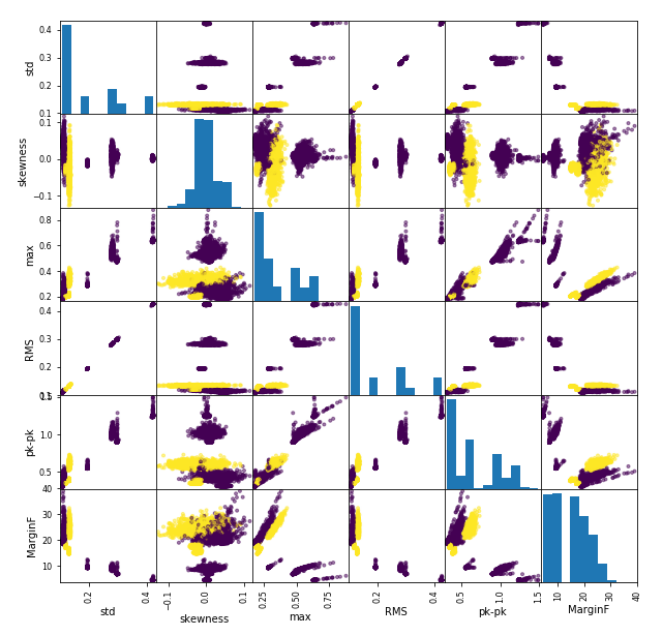
\includegraphics[width=\paperwidth]{images/6_pp}}
\caption{Pair plots for 6 features}
\end{figure}



\subsection{Best 9 features}

\subsubsection{ANN}

\begin{figure}[H]
  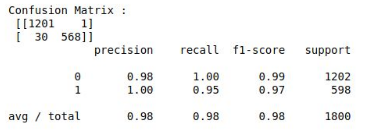
\includegraphics[height = 4cm,width= 9cm]{images/9_ANN}
\caption{Confusion Matrix for ANN}
\end{figure}

\subsubsection{SVM}

\begin{figure}[H]
  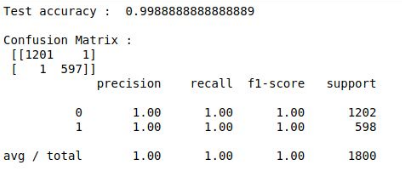
\includegraphics[height = 4cm,width= 9cm]{images/9_SVM}
\caption{Confusion Matrix for SVM}  
  \end{figure}

\subsubsection{Random Forest}

\begin{figure}[H]
  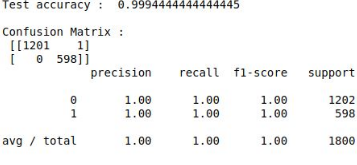
\includegraphics[height = 4cm,width= 9cm]{images/9_rand}
\caption{Confusion Matrix for Random Forest}
\end{figure}

\subsubsection{Pair Plots}

\begin{figure}[H]
  \noindent\makebox[\textwidth]{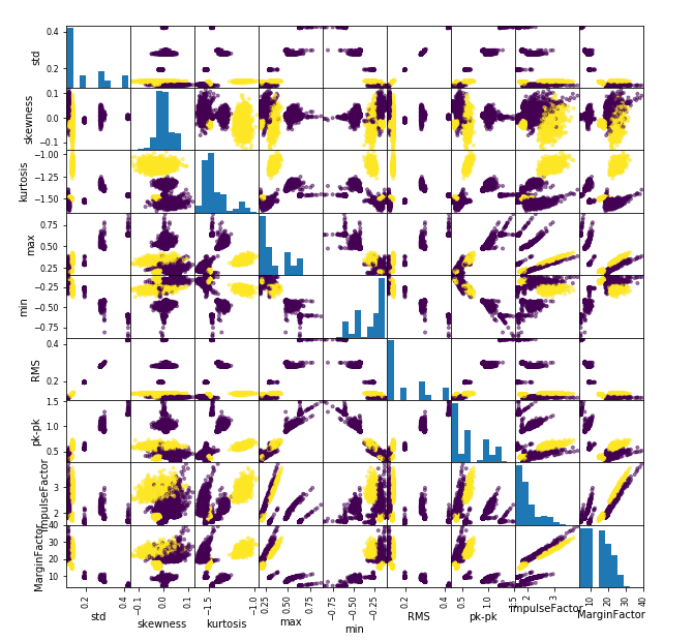
\includegraphics[width=\paperwidth]{images/9_pp}}
\caption{Pair plots for 9 features}
\end{figure}

\subsection{Best 12 features}

\subsubsection{ANN}

\begin{figure}[H]
  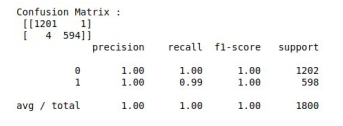
\includegraphics[height = 4cm,width= 9cm]{images/12_ANN}
\caption{Confusion Matrix for ANN}
\end{figure}

\subsubsection{SVM}

\begin{figure}[H]
  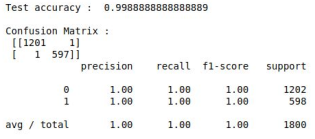
\includegraphics[height = 4cm,width= 9cm]{images/12_SVM}
\caption{Confusion Matrix for SVM}  
  \end{figure}

\subsubsection{Random Forest}

\begin{figure}[H]
  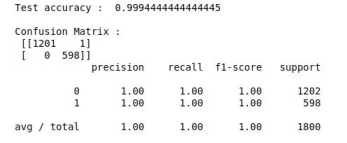
\includegraphics[height = 4cm,width= 9cm]{images/12_rand}
\caption{Confusion Matrix for Random Forest}
\end{figure}